\documentclass[journal]{IEEEtran}


% *** CITATION PACKAGES ***
\usepackage{cite}

% *** GRAPHICS RELATED PACKAGES ***
\ifCLASSINFOpdf
\usepackage[pdftex]{graphicx}
\graphicspath{{../pdf/}{../jpeg/}}
\DeclareGraphicsExtensions{.pdf,.jpeg,.png}
\else
\fi

\renewcommand{\labelenumi}{\arabic{enumi}. }
%\usepackage{enumitem}
% *** MATH PACKAGES ***
\usepackage[cmex10]{amsmath}
\def\mathbi#1{\textbf{\em #1}}
\usepackage{amssymb}
\DeclareMathOperator*{\argmax}{arg\,max}
\usepackage{comment}
\usepackage{tikz}
\newcommand*\circled[1]{\tikz[baseline=(char.base)]{
		\node[shape=circle,draw,inner sep=1pt] (char) {#1};}}

\usepackage{accents}
\newcommand{\ubar}[1]{\underaccent{\bar}{#1}}

\usepackage{algorithm}
\usepackage{algorithmic}

\usepackage{amsthm}
\newtheorem{theorem}{Theorem}[section]
\newtheorem{corollary}{Corollary}[theorem]
\newtheorem{lemma}[theorem]{Lemma}
\newtheorem*{remark}{Remark}

\usepackage{mathtools}
\DeclarePairedDelimiter\ceil{\lceil}{\rceil}
\DeclarePairedDelimiter\floor{\lfloor}{\rfloor}
\DeclarePairedDelimiter\abs{\lvert}{\rvert}


\begin{document}
\title{Transient Stability under Load Perturbation using Small Gain Theorem}
\author{Dongchan~Lee, Long~Vu and Konstantin~Turitsyn}
%\thanks{D. Lee and K. Turitsyn are with the Department of Mechanical Engineering, Massachusetts Institute of Technology, Cambridge, MA 02139, USA (email: dclee@mit.edu; turitsyn@mit.edu).}% <-this % stops a space
%\thanks{This work was supported by the NSF  awards  1554171  and  1550015 and Advanced Grid Modeling Program of the Office of Electricity within the U.S Department of Energy.}

% The paper headers
%\markboth{Submitted for publication. This version: May 2, 2017}{}
%{D. Lee}
\maketitle

%\begin{abstract}
%\end{abstract}

%\begin{IEEEkeywords}
%\end{IEEEkeywords}

\IEEEpeerreviewmaketitle


\section{Introduction}
The nonlinearities of power system equation is often dealt by bounding techniques on the nonlinear terms in the dynamic equations \cite{}. 
By finding the optimal sector bound on the nonlinearity in the system dynamics, our paper proposes a new approach to find maximum perturbation in power injections that certifies stability.

\section{Transient Stability under Load Perturbation}
In this paper, we consider the structure-preserving second order swing equation model given by
\begin{equation}
\begin{aligned}
m_k\ddot{\delta}_k+d_k\dot{\delta}_k+\sum_{\{k,j\in\mathcal{E}\}}a_{kj}\sin(\delta_k-\delta_j)&=P_k,\ k\in\mathcal{G} \\
d_k\dot{\delta}_k+\sum_{\{k,j\in\mathcal{E}\}}a_{kj}\sin(\delta_k-\delta_j)&=P_k,\ k\in\mathcal{L}
\end{aligned}
\label{eqn_swing}
\end{equation}
where $m_k$ and $d_k$ are inertia and damping of the generator $k$ in equation.$a_{kj}=V_kV_jB_kj$ where $B_kj$ is the susceptance of the transmission line connecting bus $j$ and $k$ and $V_k$ is the voltage magnitude at bus $k$. The set of generators and loads are denoted as $\mathcal{G}$ and $\mathcal{L}$ respectively, and $\mathcal{E}$ denotes the edges of the line as a pair of indices. The power injection at generators and loads will be considered as the input perturbation to the system, and output will be the generator angles, $\delta$, and frequency, $\dot{\delta}$, which should remain synchronized.

We consider large perturbations in the load $P_k=P_{k,0}+\Delta P_k, \ k\in\mathcal{L}$, and derive a provable bound on the perturbation that the system remains stable.

\noindent\textbf{Problem Formulation}: Consider a nonlinear system $\dot{x}=f(x)+u$. Find the interval $\mathcal{U}=[\underbar{$u$},\bar{u}]$ such that if $u\in\mathcal{U}\ \forall t$, then $y\in\mathcal{Y}$ where $\mathcal{Y}=[\underbar{$y$},\bar{y}]$.

While the above problem is difficult to solve for a general nonlinear system, we will consider the second order swing equation in (\ref{eqn_swing}) for the application in transient stability assessment.

\begin{remark}
As long as $\mathcal{Y}$ contains only the desirable equilibrium, the system remain stable under any disturbances $u\in\mathcal{U}$.
\end{remark}

Suppose the input perturbation and output is defined as $u\in\mathbb{R}^{n}$ and $u\in\mathbb{R}^{m}$ respectively. Let us linearize our system at the nominal operating point and let this linearized system be $G$. Then we substitute new variables to any nonlinear terms that are left in Equation \ref{eqn_swing} with $v\in\mathbb{R}^{l}$. We define $\varphi$ as the nonlinear operator that acts on a linear combination of states $w\in\mathbb{R}^{l}$, which is the input to the nonlinear term. For example, suppose we are given a system $\dot{x}=-2x+\sin(x)+u$ with nominal operating point $x_0$ and $u_0$ with output $y=x$. Then the linearized plant will be defined as $G: \dot{x}=-2x+\cos(x_0)(x-x_0)+v+u_0+\Delta u$ with $u=\Delta u$ and $\varphi: v=\sin(x)-\cos(x_0)(x-x_0)$ with $w=x-x_0$. This representation can be illustrated with Figure \ref{fig_system_w_uncertainty} where the nonlinear term is separated out into a closed-loop subsystem.

\begin{figure}[!htbp]
	\centering
	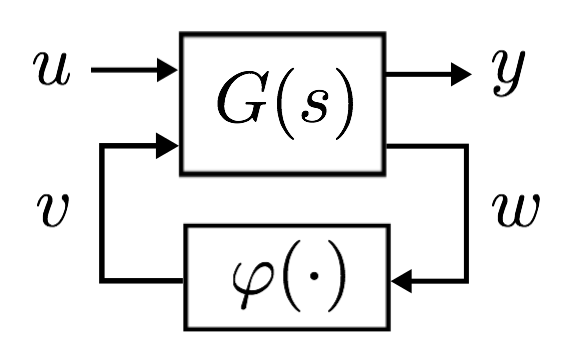
\includegraphics[width=1.5in]{picture/system_w_uncertainty.png}
	\caption{Block diagram for the system with nonlinearity.}
	\label{fig_system_w_uncertainty}
\end{figure}

Let the $\mathcal{L}2$ gain of $G$ is given by $\gamma_G\in\mathbb{R}^{(m+l)\times(n+l)}$

\begin{equation}
\gamma_G=\begin{bmatrix}
        \gamma_{G(y,u)} & \gamma_{G(y,v)} \\
        \gamma_{G(w,u)} & \gamma_{G(w,v)} \\
     \end{bmatrix}
\end{equation}
where $\gamma_{G(y,u)}\in\mathbb{R}^{m\times n}$,  $\gamma_{G(y,v)}\in\mathbb{R}^{m\times l}$,  $\gamma_{G(w,u)}\in\mathbb{R}^{l\times n}$, and  $\gamma_{G(w,v)}\in\mathbb{R}^{l\times l}$ are the components in the gain of the system. Let $\gamma_\varphi$ be the $\mathcal{L}2$ gain from the nonlinearity. Note that $\gamma_\varphi$ is a function of the bound on the input, $\max_t|w|$.

From the definition of $\mathcal{L}2$ gain, we have the following inequalities.
\begin{equation}
\max_t|y|\leq\gamma_{G(y,u)} \max_t|u|+\gamma_{G(y,v)}\max_t|v|
\label{eqn_plant_y_gain}
\end{equation}
\begin{equation}
\max_t|w|\leq\gamma_{G(w,u)} \max_t|u|+\gamma_{G(w,v)}\max_t|v|
\label{eqn_plant_w_gain}
\end{equation}
\begin{equation}
\max_t|v|\leq\gamma_\varphi \max_t|w|.
\label{eqn_nonlinearity_gain}
\end{equation}

\begin{theorem}
\textit{(Small-Gain Theorem)} The system is finite gain $\mathcal{L}$ stable if  $\gamma_G\gamma_\varphi<1$.
\end{theorem}

We substitute equation \ref{eqn_nonlinearity_gain} and $\max_t|w|=\max_t|y|$ into equation \ref{eqn_plant_w_gain},
\begin{equation}
\max_t|w|\leq\gamma_{G,u} \max_t|u|+\gamma_{G,v}\gamma_\varphi \max_t|w|
\label{eqn_w_leq_G}
\end{equation}

By rearranging,
\begin{equation}
\gamma_{G,u}^{-1}(1-\gamma_{G,v}\gamma_\varphi)\max_t|w|\leq\max_t|u|
\end{equation}

\begin{theorem}
If $\bar{u}<\gamma_{G,u}^{-1}(1-\gamma_{G,v}\gamma_\varphi)\bar{w}$ and $\gamma_{G,v}\gamma_\varphi<1$, then $\max_t|w|<\bar{w}$ for every $u$ such that $\max_t|u|<\bar{u}$.
\end{theorem}

\begin{proof}
From equation \ref{eqn_w_leq_G},
$$\max_t|w|\leq\gamma_{G,u} \max_t|u|+\gamma_{G,v}\gamma_\varphi \max_t|w|$$
$$\begin{aligned} (1-\gamma_{G,v}\gamma_\varphi)\max_t|w| &\leq\gamma_{G,u} \max_t|u|\leq\gamma_{G,u}\bar{u} \\ 
&\leq\gamma_{G,u}\gamma_{G,u}^{-1}(1-\gamma_{G,v}\gamma_\varphi)\bar{w} \\
&\leq(1-\gamma_{G,v}\gamma_\varphi)\bar{w} \end{aligned}$$
Since $1-\gamma_{G,v}\gamma_\varphi>0$, $\max_t|w|<\bar{w}$.

\end{proof}

\begin{remark}
If the trajectories of the solution is desired to stay in $\bar{y}$, then $\bar{u}=\gamma_{G,u}^{-1}(1-\gamma_{G,v}\gamma_\varphi)\bar{w}$ is the maximum input perturbation allowed to ensure the stability of the system.
\end{remark}

To find the maximum gain, the following optimization problem needs to be solved 
\begin{equation}
\begin{aligned}
& \underset{\bar{w}}{\text{maximize}} & & \gamma_{G,u}^{-1}(1-\gamma_{G,v}\gamma_\varphi(\bar{w}))\bar{w} \\
\end{aligned}
\label{eqn_opt}
\end{equation}
where $\gamma_\varphi(\bar{w})$ is a monotonically increasing function with respect to $\bar{w}$.
There are two competing effects which are
\begin{enumerate}
\item As $\bar{w}$ increases, $\gamma_\varphi$ increases. This increases the gain coming from the nonlinearities, so it reduces the certifiable range $\bar{u}$.
\item If $\bar{w}$ is too small, $\bar{u}$ is proportionally reduced according to Equation \ref{eqn_plant_w_gain}.
\end{enumerate}

\section{Sector Bound}


\begin{figure}[!htbp]
	\centering
	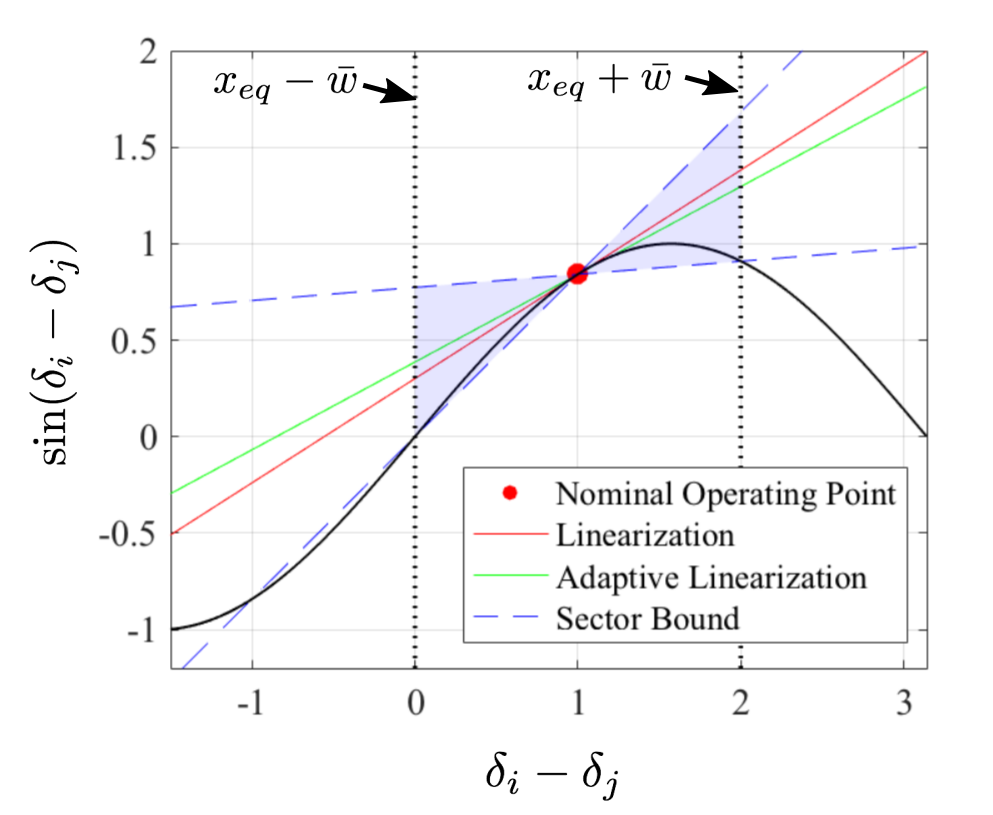
\includegraphics[width=3.2in]{picture/sector_bound.png}
	\caption{Sector bound for sin function.}
	\label{fig_sector_bound}
\end{figure}

This observation is shown in the optimization problem in (\ref{eqn_opt}) as a multiplication of monotonically increasing function $\bar{w}$ and monotonically decreasing function $(1-\gamma_{G,v}\gamma_\varphi(\bar{w}))$.

\textbf{Conjecture}: With some Lipschitz condition on $\gamma_\varphi$ or its derivative, the objective function in optimization problem \ref{eqn_opt} is a quasi-concave or even concave function of $\bar{w}$

\begin{lemma} If $g(x)$ is monotonically decreasing function with Lipschitz constant of  is 1, then $xg(x)$ is a quasi-concave function. \end{lemma}
\begin{proof} 
$$\frac{d}{dx} xg(x)=g(x)+x\frac{dg}{dx}$$
\end{proof}

Proposed solution for solving optimization problem in \ref{eqn_opt}.
\begin{enumerate}
\item Heuristic solution with gradient descent with momentum.
\item If the problem is quasi-concave function, we could solve for the gradient of the problem becoming zero since the problem is unconstrained. If the Lipschitz constant of the derivative of the objective function is less than 1, then the fixed point iteration can be applied.
\end{enumerate}

\subsection{Adaptive Linearization}
In this section, the linearization at the nominal operating point is modified to consider the bound on the uncertainties. The adaptive linearization results in less conservative bound on the input perturbation.

\section{Case Studies}
\subsection{Single Machine Example}
\begin{equation}
m\ddot{\delta}+d\dot{\delta}+a\sin\delta=P
\end{equation}

Suppose the nominal operating condition is $\delta_0$ and $P_0$. By substituting $y=\delta-\delta_0$, $w=E(\delta-\delta_0)$, $u=P-P_0$, and $v=\sin(\delta)-\cos(\delta_0)y$,
\begin{equation}
m\ddot{y}+d\dot{y}+b(v+\cos(\delta_0)y)=u
\end{equation}

In frequency domain,
\begin{equation}
\begin{aligned}
Y&=\frac{1}{ms^2+ds+a\cos(\delta_0)}U-\frac{b}{ms^2+ds+a\cos(\delta_0)}V \\
&=G_uU+G_vV
\end{aligned}
\end{equation}

%\appendices

\ifCLASSOPTIONcaptionsoff
\newpage
\fi

\bibliographystyle{IEEEtran}
\bibliography{references}
\nocite{*} 

\end{document}







